\chapter{What Drives State-Sponsored Violence?: Evidence from Extreme Bounds Analysis and Ensemble Learning Models}
\label{chap:killings}

\section{Introduction}
\label{sec:intro4}

Since the end of World War II, mass killings, genocides, and politicides have claimed over 34.5 million lives \citep{marshall2017pitf}.\footnote{Genocide and politicide are the attempted intentional destruction of communal or political groups, respectively \citep[see][]{harff1988toward}. Mass killing includes these atrocities, as well as attacks against civilians that result in at least 1,000 deaths but are not intended to destroy a particular group \citep[see][]{ulfelder2008assessing}. While some conflate the logic of these types of atrocities \citep[e.g.,][]{stanton2015regulating, valentino2004draining}, others claim genocide and politicide follow a different logic from other forms of government violence \citep{kalyvas2006logic,stanton2015regulating}. Note that these arguments focus on the logic of the violence, not legal definitions that separate and prioritise genocide as the crime of crimes \citep[see][]{schabas2000genocide}.} The international community has responded with an effort to prevent further state-sponsored mass murder by strengthening laws against crimes against humanity, genocide, and war crimes. It formed \textit{ad hoc}, hybrid, and a permanent criminal court to punish and deter future atrocities. Furthermore, the United Nations established a Special Adviser on the Prevention of Genocide and recognised its members’ responsibility to protect civilian populations within and outside their own borders. Yet, such atrocities still occur. Recently, President al-Assad of Syria has massacred tens of thousands of civilians during the Syrian Civil War \citep{goldman2017nyt}. Similarly, South Sudan's President Kiir is actively starving and killing civilians from dissident and rival tribes \citep{nichols2017reuters}. While there is some evidence that such atrocities may be declining since the Cold War \citep{valentino2014we}, the international community has been far from successful in realising slogans like ``Never Again'' and ``Not on My Watch'' \citep{cheadle2007not}.

Ultimately, successful prevention requires us to understand why these atrocities occur. In this vein, the academic community has laboured tremendously to establish evidence-based theories as to why governments engage in brutality against their civilian populations. Indeed, since 1995, there have been over 45 quantitative political science articles focused on explaining government-sponsored killing of civilians. Note, this number does not consider the myriad other books, qualitative articles, and non-political science research conducted into this matter. Overall, the mass violence literature generally agrees that as threat increases, so does the likelihood of atrocity, if the costs to such violence are not prohibitive. However, there is little consensus on what factors influence the level of threat or costs a regime faces. Part of the reason for this uncertainty is that scholars use very different model specifications when testing their arguments. Examining the quantitative literature on government violence against civilians, we found that in 45 studies, scholars used nearly 180 measurements to capture roughly 30 key concepts related to threat and costs. While models should be constructed specifically to test particular arguments, one concern is that small changes in model specification could in influence the robustness of empirical results and the inferences that we can draw from these results.

To overcome these limitations and provide a better understanding of government atrocity, we employ extreme bounds analysis and random forests to identify the most robust determinants of state-sponsored atrocities. Our approach is similar to \cite{hegre2006sensitivity} seminal analysis on the causes of civil war onset, but we provide additional tests to check which variables are able to predict out-of-sample cases of mass violence during both peacetime and wartime. In conducting this analysis, we address three debates in the mass violence literature:

\begin{enumerate}
    \item Why do some governments engage in mass killings, genocides, or politicides? This is the primary question asked by advocates, policymakers, and scholars in this field of research. It is also the question that the 45 studies mentioned above each attempt to answer.
    \item Does the logic underpinning government decision-making follow different patterns during peacetime and wartime. Recent research suggests that government atrocity occurs predominantly during periods of civil war \citep{harff2003no} which has led some scholars to restrict their analyses to only periods of civil war \citep[e.g.,][]{colaresi2008kill, valentino2004draining} or concentrate on predicting both the onset of civil war and atrocity \citep{goldsmith2013forecasting}. Yet, others estimate models of all country-year \citep[e.g.,][]{krain1997state, montalvo2008discrete}, raising questions of how well these studies speak to each other.
    \item Is there a difference in logic between those atrocities labelled as genocide or politicide, compared to other mass killings? While the Political Instability Task Force \citep{marshall2017pitf} provides the most widely used data on government atrocity, these data are limited only to cases of genocide and politicide. Others provide data with much more lenient inclusion criteria \citep[e.g.,][]{eck2007one, rummel1995democracy, stanton2015regulating, ulfelder2012forecasting}. These differences in definition of atrocity have led to divergent results, raising questions about important determinants of government behaviour \citep[for discussion, see][]{uzonyi2016domestic, wayman2010explaining}.
\end{enumerate}

Our analysis tests the sensitivity of 40 variables on a sample of 177 countries from 1945 to 2013. We find that GDP \textit{per capita}, democratic regimes, and the post-Cold War period are negatively associated with mass killings, whereas previous political turmoil increases the risk of such violence. In contrast, the distributed random forest algorithm indicates that years since the last episode of mass violence, GDP \textit{per capita}, urban population, openness to trade, and the number of military personnel make the greatest contribution to our models’ out-of-sample predictive power. While we discuss the importance of these findings in more detail later in this article, a few notes are imperative to make here. First, in some ways, these findings confirm previous research–unstable countries are more likely to witness the regime employ atrocity \citep[e.g.,]{goldsmith2013forecasting,harff2003no,krain1997state}.  However, many of the factors scholars often cite as observable indicators of such instability--regime transitions, coups d'état, the presence of militias, etc.--are not good proxies for instability. Thus, policymakers may be looking for the incorrect signs of impending atrocity when seeking to prevent its onset. Second, these findings raise concerns about policy options for preventing violence against civilians. If our conclusion is that unstable countries are violent, then preventing atrocity likely requires significant investments of time and resources in state-building, which is often politically and practically unfeasible \citep{doyle2006making}. Lastly, our findings are robust to a myriad of specifications, functional forms, and additional tests as we describe below. This analysis contributes significantly to the political violence literature by highlighting the parsimonious nature of the logic behind government atrocity and clearing away much of the empirical clutter surrounding this conclusion. 

\section{Empirical Methods}
\label{sec:methods4}

We employ two methods to test the robustness of the potential determinants of state-led violence. First, we use a variant of extreme bounds analysis (EBA) to check the statistical significance of 35 explanatory variables cited in the academic literature.\footnote{The complete list of variables included in this article is available in the online appendix. Our selection procedure was as follows. We included all variables that appeared in at least two two quantitative papers on mass killings which employed logit or probit models in a global sample. We considered only published articles in our list.} Researchers have employed the EBA to assess the sensitivity of the determinants of civil war \citep{hegre2006sensitivity}, coups d'état \citep{gassebner2016expect}, democratisation \citep{gassebner2013extreme}, economic growth \citep{levine1992sensitivity, sala1997just, sturm2005determinants}, nuclear deterrence \citep{bell2015examining}, political repression \citep{hafner2005right}, and state corruption \citep{serra2006empirical}. The method is particularly useful when there is no consensus about which covariates belong in the ``true'' regression model \citep[178]{sala1997just} and scholars worry that omitted or unnecessary predictors could bias the parameter estimates \citep[60]{angrist2008mostly, clarke2005phantom, elwert2014endogenous, spector2011methodological}. By combining a large set of regression models into a single posterior distribution, the EBA reduces the uncertainty associated with the \textit{ad hoc} selection of predictors and provides an intuitive way of assessing the relative strength of the statistical findings \citep{leamer1985sensitivity, sala1997just}.

Second, we employ distributed random forest (DRF) \citep{breiman2001random, h2o2017} to measure the predictive power of our set of independent variables. Random forest has been widely used in the machine learning community and consistently ranks among the best algorithms for predicting structured data.\footnote{Random forests, gradient boosting machines, and neural networks have won the highest number of competitions on Kaggle, a crowd-sourced platform for predictive modelling \citep{carpenter2011may}. While data analysts prefer neural networks for problems with a high number of hidden features such as image recognition, random forest and gradient boosting are the top choices for dealing with tabular data. See: \href{https://www.kaggle.com/antgoldbloom/what-algorithms-are-most-successful-on-kaggle}{https://www.kaggle.com/antgoldbloom/what-algorithms-are-most-successful-on-kaggle} (access: December 2017).} DRF does not require distribution assumptions, can be used with any type of response variables, and are able to automatically detect nonlinear relationships between correlates \citep{fernandez2014we, hill2014empirical, jones2015exploratory, muchlinski2015comparing}. Moreover, unlike neural networks and other deep learning algorithms \citep{castelvecchi2016can,rojas2013neural,shwartz2017opening}, the output of DRF models can be interpreted meaningfully. DRF offers precise estimates of the predictive ability of each individual variable, and it also allows researchers to graphically visualise the marginal effect of the covariates on the response variable \citep{friedman2001greedy,friedman2001elements,goldstein2015peeking}.


\subsection{Extreme Bounds Analysis}
\label{subsec:eba}

The main purpose of the extreme bounds analysis is to estimate the distribution of coefficients of each predictor $x$ in an exhaustive combination of regression models with $y$ as a dependent variable. \cite[308]{leamer1985sensitivity} argued that the EBA could certify scholars that ``minor changes in the list of variables do not alter fundamentally the conclusions, nor does a slight re-weighting of observations, nor correction for dependence among observations, etcetera, etcetera.'' He proposed that ``sturdy'' variables are those whose minimum and maximum of their coefficient distribution have the same sign and are situated at a distance from zero. If we are to use the conventional value of $p < 0.05$, the mean of the variable coefficients' distribution should be located at least $1.96$ standard deviations away from zero. 

Leamer's criterion is intuitive, but other authors contend it is too strict for most social science applications. \cite{sala1997just} argued that Leamer's EBA would increase the number of false negatives; in other words, it would classify as fragile covariates that are truly associated with the response. If a given variable of interest appears as both positive and negative in the literature, it is likely that after a large a number of regressions the predictor will change signs and therefore be deemed fragile \citep[179]{sala1997just}. Sala-i-Martin then offered a less stringent version of the EBA in which researchers analyse the full distribution of point estimates instead of relying only on the coefficients' extreme bounds. 

In this paper, we follow his advice and consider the whole range of values of $CDF(0)$. We choose to use the whole distribution because the aggregate $CDF(0)$ allows us to move away from a binary indicator of robustness, the one we obtain with Leamer's extreme bounds, and present the estimations with their appropriate degrees of confidence \citep[179]{sala1997just}\footnote{As \citet[179]{sala1997just} describes, ``if 95 percent of the density function for the estimates of $\beta_{1}$ lies to the right of zero and only 52 percent of the density function for $\beta_{2}$  lies to the right of zero, one will probably think of variable 1 as being more likely to be correlated with [a dependent variable $Y$] than variable 2.''}. Our main focus is the percentage of the variable's cumulative distribution function that is smaller or greater than zero. We do not assume that the CDF has a normal distribution: Many of our coefficients do not follow a normal distribution, so the generic model provides a better fit to our data. We specify our models as follows:

\begin{equation}
\text{\textit{Mass Killing Onset}}_{it} = \beta_{M}M_{it} + \beta_{F}F_{it} + \beta_{Z}Z_{it} + v_{it}
\end{equation}

Our main dependent variable is \textit{Mass Killing Onset}, which denotes the onset of government-sponsored killings. It was coded by \cite{ulfelder2008assessing}. The authors define a mass killing as ``any event in which the actions of state agents result in the intentional death of at least 1,000 noncombatants from a discrete group in a period of sustained violence'' \citep[2]{ulfelder2008assessing}. In our additional tests, we also estimate the models with an indicator of Genocide/Politicide Onset by \cite{harff2003no}. We prefer the first measure not only because it provides a clear numerical threshold that separates mass killings from low-level violence, but also because it focuses on the killing of members of a given community, not on the absolute number of deaths. 

The indices $i$ and $t$ indicate country and year, respectively. $M$ is a set of three covariates that are included in every model due to their prominence in the literature \citep{levine1992vale}. In our analysis, we have added the natural logarithm of the GDP \textit{per capita} to control for income, the Polity IV index to control for level of democracy, and a linear time trend since the last episode of government-led atrocity to account for temporal dependence. $F$ denotes a vector of variables of interest, and $Z$ is a vector of other control variables in addition to those included in $M$. Our first model includes the variable of interest, 3 additional control variables, and 3 covariates that appear in every regression. $v$ is the error term. In practice, however, since we are interested in the effect of all variables in the data set and we do not have true control variables except from $M$, in our case $F$ and $Z$ are interchangeable. Following \citet[514]{hegre2006sensitivity}, the independent variables have been lagged one year to reduce the risk of endogeneity. Although our dependent variable is dichotomous, we use linear probability models in our main analysis. As argued by \citet[298]{gassebner2016expect}, linear probability models are less prone to convergence problems, their estimation is faster, and their results can be readily interpreted. While we do employ logistic and probit models as robustness tests, we report the coefficients of the linear probability models as our primary estimates. Moreover, since the data are grouped into countries, we use cluster-robust standard errors to control for within-cluster error correlation.
 
One of the shortcomings of our data is that some variables are strongly correlated. For instance, we include the Correlates of War's Composite Index of National Capability (\textit{CINC}), which is composed by six different variables \citep{cow2017cinc,singer1988reconstructing}.\footnote{For more information about the CINC index, please refer to the Correlates of War website: \href{http://www.correlatesofwar.org/data-sets/national-material-capabilities/national-material-capabilities-v4-0}{http://www.correlatesofwar.org/data-sets/national-material-capabilities/national-material-capabilities-v4-0} (access: December 2017).} Multicollinearity would induce bias to our estimates, so we add CINC and three of its components\footnote{The variables correspond to the ratio between the national and the global values.} -- military expenditure, military personnel, and total population -- as mutually exclusive variables. These predictors are not included in the same regression model to avoid collinearity issues.
 
We add another set of mutually exclusive variables to reduce collinearity. There are three covariates that denote ongoing civil conflicts: one measured by the Uppsala Conflict Data Program \citep{allansson2017organized,gleditsch2002armed}, another coded by the Correlates of War \citep{sarkees2010resort}, and a third indicating the onset of ethnic conflict as coded by \citet{cederman2010ethnic}. We include only one of these measures at a time. 
 
As a last precaution against collinearity, we place a limit on the Variance Inflation Factor (\textit{VIF}) of all regression coefficients. The VIF estimates how much of the variance of each predictor is dependent on the other covariates in a model. A VIF of 1 indicates that the predictor is uncorrelated with the remaining covariates. The VIF limits are often arbitrary \citep{bell2015examining,o2007caution}, thus we use a moderately conservative VIF of 7 in our estimates. As robustness tests, we run the same models with different VIF cut-offs and without restriction.

Two variables were omitted from the EBA models but included in the machine learning models below. The first is \textit{democracy}, a dummy variable that indicates whether the country is a has a Polity IV score equal or higher than 5. The second is \textit{interstate war}, a binary covariate measuring if the country is at war in a given year \citep{sarkees2010resort}. We have decided to omit democracy because of its obvious correlation with the Polity measure and interstate war due to its correlation with our dependent variables. The EBA models do not converge if those variables are added. Since this problem does not affect machine learning algorithms, the two variables were included in the second set of estimations.

Lastly, we depart slightly from Sala-i-Martin's suggested method and do not assign weights to the EBA. Although he recommends using goodness-of-fit measures to construct regression weights, we agree with \citet{sturm2002robust} and \citet[299]{gassebner2016expect} and use the unweighted version of the CDF instead. Goodness-of-fit indicators are not equivalent to the probability of a given model being true \citep{achen1977measuring,anscombe1973graphs,king1986not}, and the weights constructed this way are not invariant to transformations in the dependent variable. Moreover, our data set has a number of missing observations, so that model comparison would be misleading \citep{lall2016multiple}. Thus, the results below are for unweighted estimations. 

\subsection{Distributed Random Forest}
\label{sub:drf}

Random forest is a machine learning algorithm that consists of a combination of individual decision trees. In a classification problem, each decision tree uses a vector of covariates to split the dependent variable into two increasingly homogeneous parts \citep{breiman2001statistical}. However, decision trees are prone to overfitting, i.e., they match the original data set so closely that they tend to perform poorly with new data \citep{dietterich1995comparison,ho1998random}. Random forest, in contrast, avoids this issue by growing a decision tree only to a bootstrap sample of the original data, selecting random features at each split, then aggregating the different trees into a single prediction. If the independent variable is continuous, the algorithm will simply choose the average value of the predictions as the best candidate; if the covariate is discrete, the majority class will be employed. The simple procedure of leaving out some data points and growing separate trees with a random subset of covariates is sufficient to eliminate the risk of overfitting \citep[9-10]{jones2015exploratory}.

Random forest has many desirable properties, such as ``highly accurate predictions, robustness to noise and outliers, internally unbiased estimate of the generalisation error, efficient computation, and the ability to handle large dimensions and many predictors'' \citep[7]{muchlinski2015comparing}. Thus, random forest allows the researcher to estimate very flexible models with minimal assumptions. Unlike parametric methods such as ordinary least squares or logistic regressions, the analyst does not have to impose any distributional form to the data-generating process. As a result, random forest is able to effectively uncover complex, nonlinear interaction effects in the data without prespecification \citep{jones2015exploratory,strobl2007bias}.

The algorithm can also deal with heavily imbalanced data. Researchers can balance the classes of their response variable by assigning different sampling probability to each category. This enables the algorithm to make accurate prediction for rare events without adding prior distributions or resorting to subjective modelling choices \citep{chen2004using,del2014use,muchlinski2015comparing}.

In this paper we use distributed random forest (DRF) to model our data \citep{h2o2017}. The DRF is essentially identical to original random forest algorithm, but it has two additional features that are useful for our purposes. Firstly, DRF is optimised for big data, as it grows decision trees on separate cores to speed up computation time. Secondly, in DRF, non-observed cases are not assumed to be missing at random, but rather as values that contain information in themselves. When building decision trees, DRF treats the missing observations as a separate category that can go either left or right. This is a more conservative approach than assuming that missing cases fit into an underlying parametric distribution.\footnote{For more information about how the distributed random forest algorithm deals with missing observations, please refer to: \href{http://docs.h2o.ai/h2o/latest-stable/h2o-docs/data-science/drf.html}{http://docs.h2o.ai/h2o/latest-stable/h2o-docs/data-science/drf.html} (access: December 2017).}

The DRF has a series of hyperparameters that can be tuned to improve the algorithm's predictive performance. For instance, users can control the number of decision trees in each iteration, how deep trees should grow, which performance metric to adopt, whether to balance classes or to use cross-validation, and many other options. The interaction between parameters is generally complex and may involve thousands of potential combinations. As an example, a researcher interested in four parameters with 10 possible values each would have to estimate 10,000 models before deciding which is the most efficient one. Also, machine learning parameters are sensitive to the data at hand; so what seems an optimal solution for one problem cannot be readily implemented in another data set \citep{genuer2008random,goldstein2010application,jones2015exploratory}.

To address this issue, we have adopted an automated procedure to select the model parameters. We perform a grid search where the algorithm starts with a random combination of parameters, jumps to another randomly-chosen set, and then stops after it reaches a certain threshold \citep[123]{cook2017h2o}. We follow the literature on predictive political science and use the area under the ROC curve (AUC) as our model evaluation metric \citep[e.g.,][]{clayton2014will,hill2014empirical,ward2010perils,ward2013learning,weidmann2010predicting}. We set the metric as follows: If five random models had not increased the AUC by at least in 0.1\% comparing to the previous ones, the algorithm considers the result to be optimal. We set the maximum number of models to 1,000.

We have added several parameters to the grid search. The first is the number of independent trees to grow in each random forest model. The starting values are 256, 512, and 1024 trees. The machine learning literature does not provide a heuristic on how large a random forest should be, but \citet[166]{oshiro2012many} affirm that ``from 128 trees there is no more significant difference between the forests using 256, 512, 1024, 2048 and 4096 trees.'' We employ a more conservative approach and start from a higher value that the authors suggest as adding more trees do not reduce prediction accuracy \citep[7]{breiman2001statistical}. However, we find little evidence that the number of trees makes a noticeable difference to the estimations.

The depth of each decision tree also influences the algorithm performance. Deeper trees indicate more complex models, and in general they provide a better fit to the data. Nevertheless, this complexity comes at the risk of overfitting, so deeper trees are not necessarily the most adequate solution for every model \citep[596]{friedman2001greedy,segal2004machine}. In this article, we let the algorithm decide among using 10, 20, or 40 levels for each tree. In our view, these number offer a good balance between parsimony and complexity.

We test whether having balanced classes of our dependent variable (mass killing onset) affects the predictive ability of the model. Since the response measure is heavily imbalanced, oversampling the positive responses could potentially improve our results \citep{chawla2004special,del2014use,japkowicz2002class}. Somewhat unexpectedly, DRF had a better fit using unbalanced classes, which is the result we report in the next section.

We also vary how many variables should be considered for each split in the data. The DRF's default is to use $\sqrt{p}$, where p is the number of columns in the data set. As we have 34 covariates of interest, we have selected 5, 6 and 7 variables per split. The DRF uses a majority voting procedure to select which variable is most important. Additionally, the algorithm chooses the percentage of the training set to be modelled by each tree. The default option is 63.2\%, but we include the options of using 50\% and 100\% of the data. Similarly, we give a range of options for choosing how many columns will be included in each tree. The algorithm can randomly choose among 50\%, 90\% or 100\% of the independent variables when estimating a decision tree.

Finally, we use four types of histogram to find optimal split points for each independent variable. Decision trees consider every value of a given independent variable as a potential candidate for a split in the training data. This process is notably time-consuming, and computation time can be significantly reduced at little loss of precision by taking discrete values of the predictor distribution. The DRF algorithm offers four choices of histogram selection and we include all of them in our estimations.

\section{Results}
\label{sec:results4}

Table \ref{tab:eba1} summarises our main EBA results with Ulfelder and Valentino's \citeyear{ulfelder2008assessing} \textit{Mass Killing Onset} as the dependent variable. The table shows the average coefficient estimate of all regressions for each robust variable along with their mean standard deviations.\footnote{A list of all independent variables and coding rules are available in the online appendix.} The table also displays the percentage of regressions that are statistically significant at the 90\% level. $CDF(0)$ represents the cumulative distribution function, which is the area of the distribution that falls above or below zero.\footnote{We show whichever area is the largest. The sign of the average $\beta$ coefficient indicates if most of the cumulative distribution is located above or below zero.} This is our main statistic of interest, and we consider a covariate to be robust if it has a $CDF(0)$ of 0.9 or higher \citep[181]{sala1997just}. Lastly, we report the number of estimated regressions models which included each variable.

\begin{table}[H]
\centering
\begin{tabular}{lrrrrr}
\hline
\textbf{Variable} & \textbf{Avg. $\beta$} & \textbf{Avg. SE} & \textbf{$\%$ Sig.} & \textbf{CDF(0)} & \textbf{Models} \\ \hline
\textit{Base variables} &  &  &  &  &  \\
Log GDP per capita & -0.0091 & 0.0052 & 76.055 & 0.9335 & 226707 \\
 &  &  &  &  &  \\
\textit{Additional variables} &  &  &  &  &  \\
Post-Cold War years & -0.0133 & 0.0085 & 72.845 & 0.9472 & 35614 \\
UCDP civil war onset & 0.0529 & 0.0321 & 52.378 & 0.9441 & 20854 \\
Previous riots & 0.0140 & 0.0100 & 56.242 & 0.9216 & 35614 \\
UCDP ongoing civil war & 0.0172 & 0.0115 & 65.652 & 0.9092 & 20854 \\
Ethnic diversity (ELF) & 0.0184 & 0.0137 & 56.674 & 0.9050 & 35614 \\
Polity IV squared & -0.0002 & 0.0001 & 61.206 & 0.9031 & 35614 \\ \hline
\end{tabular}
\caption{Extreme Bounds Analysis -- Mass Killings (robust variables only)}
\label{tab:eba1}
\end{table}

Seven variables pass our EBA criteria. Three variables decrease the likelihood of mass killings. First, as widely suggested in the literature, the natural logarithm of GDP per capita is robustly associated with the onset of mass killings 
\citep[e.g.,][]{besanccon2005relative, easterly2006development,esteban2015strategic}. In our models, GDP per capita has a negative effect on onset risk is statistically significant in 76\% of the models. Second, the post-Cold War years are correlated with lower levels of government violence. Despite eventual outbreaks of large-scale attacks against civilians \citep[e.g.,][]{prunier2005darfur,tatum2010genocide,waldorf2009revisiting}, after 1991 these events have become less prevalent. Indeed, this finding is in line with several studies that point to a general decline in violence over the last decades, including riots, civil wars, and urban crime \citep{eisner2003long,pinker2011better}. The third variable negatively correlated with mass killings is the squared term of the Polity IV political regime index. Although the linear Polity IV indicator does not reach our threshold for significance, about 90\% of the distribution area of Polity IV squared is located below zero. This finding points to a nonlinear relationship between political regime and mass killings, thus providing further evidence that democracy reduces state-sponsored violence \citep{rost2013will,rummel1995democracy} and that regimes that mix democratic with autocratic features have the highest risk of conflict \citep{hegre2001toward,mitchell2013domestic,muchlinski2014grievances,regan2010changing}.

Four variables are positively associated with Ulfelder and Valentino's (\citeyear{ulfelder2008assessing}) indicator of state-sponsored violence. The onset and continuation of civil wars are correlated with mass killings, but only when we employ the UCDP measures of violent conflict. We find no effect for the variables compiled by the Correlates of War project or \cite{cederman2010ethnic}. Coding choices likely account for this difference, and the result is robust to a myriad of specifications. Former instances of political turmoil also have a positive coefficient in our models. Countries with a previous history of riots are more prone to state violence, which suggests that government repression is path dependent 
\citep[e.g.,][]{gurr2000peoples,harff2003no,krain1997state,nyseth2017re}. Our results also show that a higher levels of ethnic diversity increase the likelihood of atrocities against civilians. Nevertheless, the variable does not pass all additional tests we implement below and the sturdiness of this finding remains open to question. The uncertainty about the impact of ELF on mass killings is also reflected in the literature. As \citet[237]{hoeffler2016development} points out, \citet{rummel1995democracy} reports that ELF is not statistically significant in his models, \citet{wood2014opportunities} finds a negative relationship and \citet{querido2009state} finds a positive one. Our analysis does not offer a definitive answer for this question either.

A different set of variables reach significance if we only consider mass killings that occur during civil wars. We ran the models on three indicators of violent armed conflict. The first is the civil war measure by the Uppsala Conflict Database Program  (\citeyear{allansson2017organized,gleditsch2002armed}). Here, two variables meet our criteria for robustness, Post-Cold War years and conflicts with territorial aims, both negatively correlated with mass killing onset. When we limit our analysis to cases marked as civil wars by the Correlates of War project, years since the last mass killing episode, previous riots, former human rights abuses, and ethnic diversity appear have a positive effect on the outcome. Rather surprisingly, the presence of militias has a negative effect on genocides and politicides. Finally, our model using ethnic civil war shows similar results: Militias have a negative impact on the likelihood of mass killings during ethnic conflict, as do conflicts over territorial aims. This finding is in contradiction with previous research \citep{koren2017means} and is deserving of further exploration. Overall, these results suggest two takeaways. First, the determinants of mass killing onset during peacetime and wartime are different from each other. While there are more restraints on atrocities during peacetime, these restraints fail once fighting begins. This raises particularly interesting questions about the pacifying nature of democracy. Second, how civil wars are classified significantly alters the results produced. This raises concerns for scholars about making claims based on only one data set.

\begin{table}[H]
\centering
\begin{tabular}{lrrrrr}
\hline
\textbf{Variable} & \textbf{Avg. $\beta$} & \textbf{Avg. SE} & \textbf{$\%$ Sig.} & \textbf{CDF(0)} & \textbf{Models} \\ \hline
\textit{Base variables} &  &  &  &  &  \\
Log GDP per capita & -0.0091 & 0.0052 & 76.055 & 0.9335 & 226707 \\
 &  &  &  &  &  \\
\textit{Additional variables} &  &  &  &  &  \\
Post-Cold War years & -0.0133 & 0.0085 & 72.845 & 0.9472 & 35614 \\
UCDP civil war onset & 0.0529 & 0.0321 & 52.378 & 0.9441 & 20854 \\
Previous riots & 0.0140 & 0.0100 & 56.242 & 0.9216 & 35614 \\
UCDP ongoing civil war & 0.0172 & 0.0115 & 65.652 & 0.9092 & 20854 \\
Ethnic diversity (ELF) & 0.0184 & 0.0137 & 56.674 & 0.9050 & 35614 \\
Polity IV squared & -0.0002 & 0.0001 & 61.206 & 0.9031 & 35614 \\ \hline
\end{tabular}
\caption{Extreme Bounds Analysis -- Mass Killings (robust variables only)}
\label{tab:eba1}
\end{table}

The random forest models confirm some of the main findings of the EBA, yet they also show some interesting prediction patterns. Figure \ref{fig:drfuv} presents the six most important predictors of state-sponsored violence in out-of-sample tests. Overall, the machine learning estimations have a good fit, with an AUC of about 0.8 in the test samples.

However, the findings should be interpreted with caution since variable importance metrics are sensitive to the choice of random seed numbers. But despite that expected variation, the results in the random forest models are quite stable even when estimated with different random seeds. 

\begin{figure}[h]
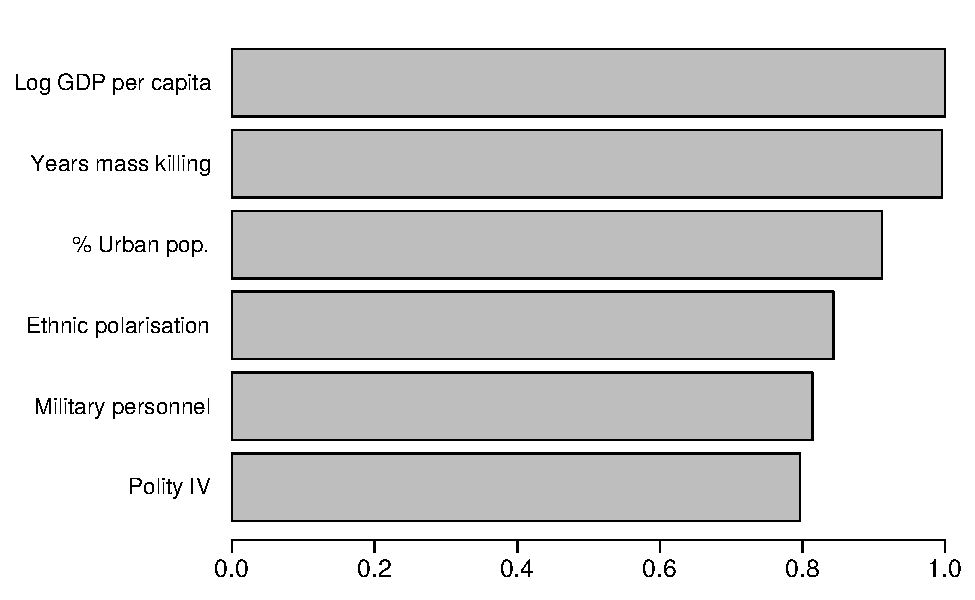
\includegraphics[width=.9\textwidth, height=8cm]{images/drf.pdf}
\caption{Distributed Random Forest -- Variable Importance (scaled)}
\label{fig:drfuv}
\end{figure}

We see that the most important predictor in our models is the natural log of GDP per capita. This confirms the findings of the EBA model. Years since the last mass killing episode has a nonlinear relationship with large-scale violence: The likelihood of renewed genocides is small in the first years, although it increases slightly over the next decades. The percentage of urban population exhibits a similar pattern. Rural areas are less prone to mass killings, yet the probability of such events rise according to a country’s level of urbanisation. We understand both GDP per capita and percentage of urban population as proxies for state capacity. Conducting a mass killing campaign demands some minimal level of military hierarchy and resources, and countries that are overwhelmingly rural are probably less able to amass the human and physical capital required to conduct such task. Furthermore, urban population tend to be less dispersed, what facilitates a large attack by government forces. 

\vspace{.5cm}

\begin{figure}[h!]
\begin{center}
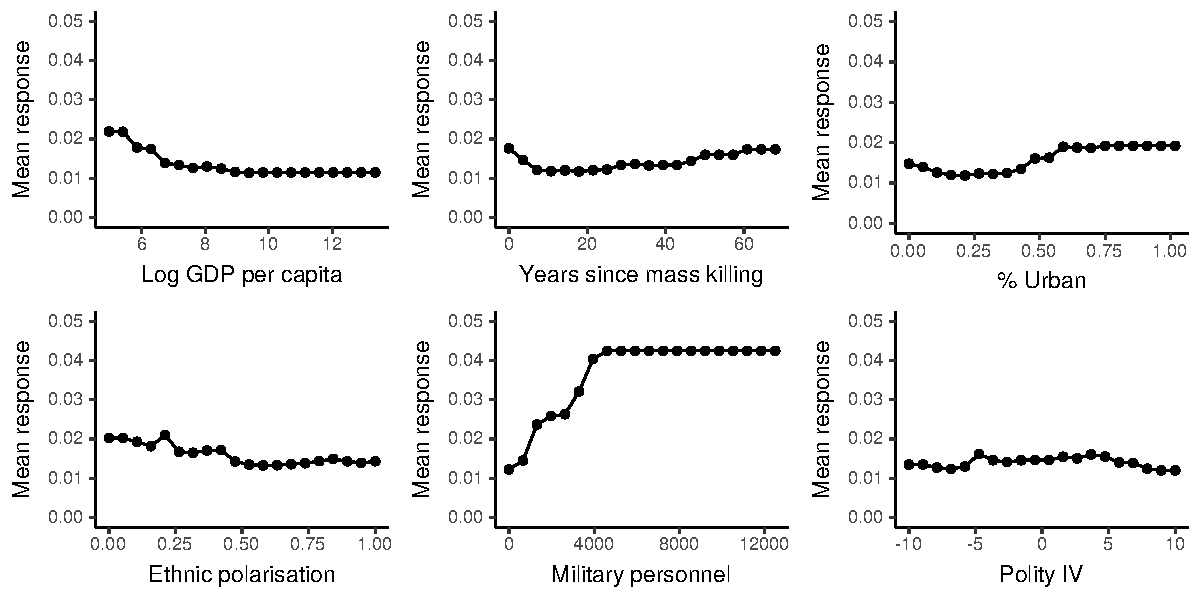
\includegraphics[width=\textwidth, height=9cm]{images/drfdpp.pdf}
\caption{Distributed Random Forest -- Partial Dependence Plots}
\label{fig:drfdpp}
\end{center}
\end{figure}

The ethnic polarisation variable indicates that countries in which a large share of the population is excluded from politically relevant positions, the lower the probability of a mass killing. Groups that manage to control the state apparatus rarely face dangerous opposition movements, and as such they rarely resort to mass violence to impose their rule over the population. Next, the size of the military personnel substantially increases the likelihood of state-sponsored violence. While small and weak states tend to be more prone to civil war and other types of conflict \citep{collier2004greed,fearon2003ethnicity}, they are less likely to experience one-sided state violence. Lastly, the Polity IV index shows that mixed regimes have a higher likelihood of atrocity, and democracies tend to have lower levels of state-led violence.

With respect to mass atrocities that occur during armed conflicts, we see that log GDP per capita and years since mass killings are again relevant predictors. Additionally, both covariates are among the 10 most important predictors in the three models. The results obtained with the UCDP civil war data are broadly similar to those of the previous model, but it highlights that total battle deaths is the predictor that has a noticeable impact on mass killings onset. The partial dependence graph shows a large positive effect along the curve, with a pronounced jump at around 200,000 deaths. 

\vspace{1cm}

\begin{figure}[h!]
\begin{center}
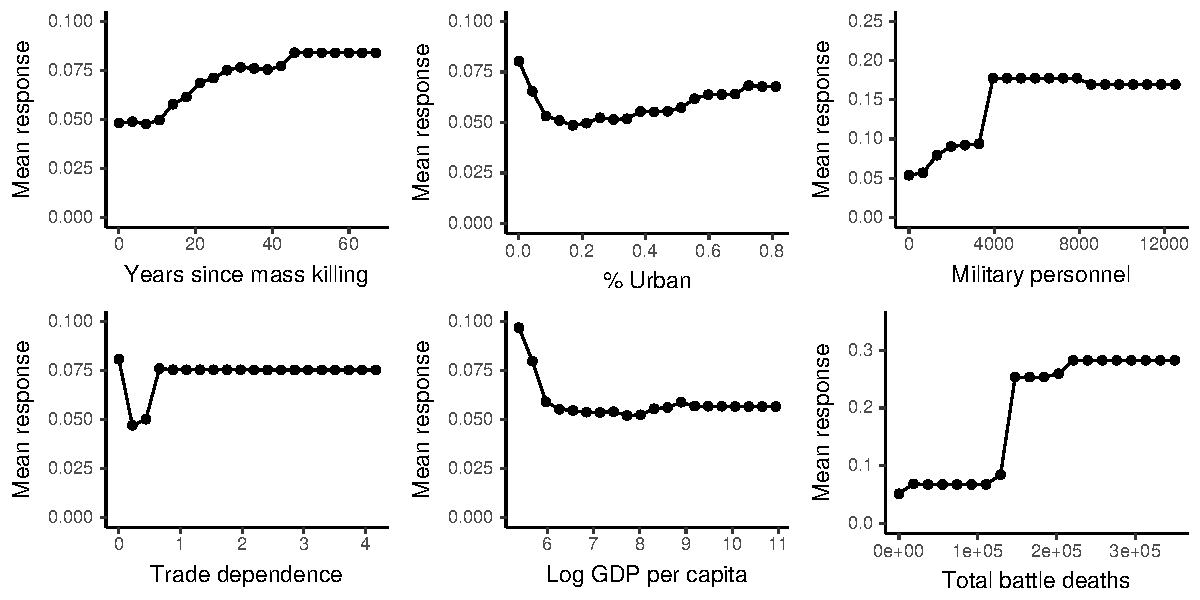
\includegraphics[width=\textwidth, height=9cm]{images/drfdpp2.pdf}
\caption{Partial Dependence Plots -- Mass Killings during Civil Wars (UCDP data)}
\label{fig:drfdpp2}
\end{center}
\end{figure}


\begin{figure}[h!]
\begin{center}
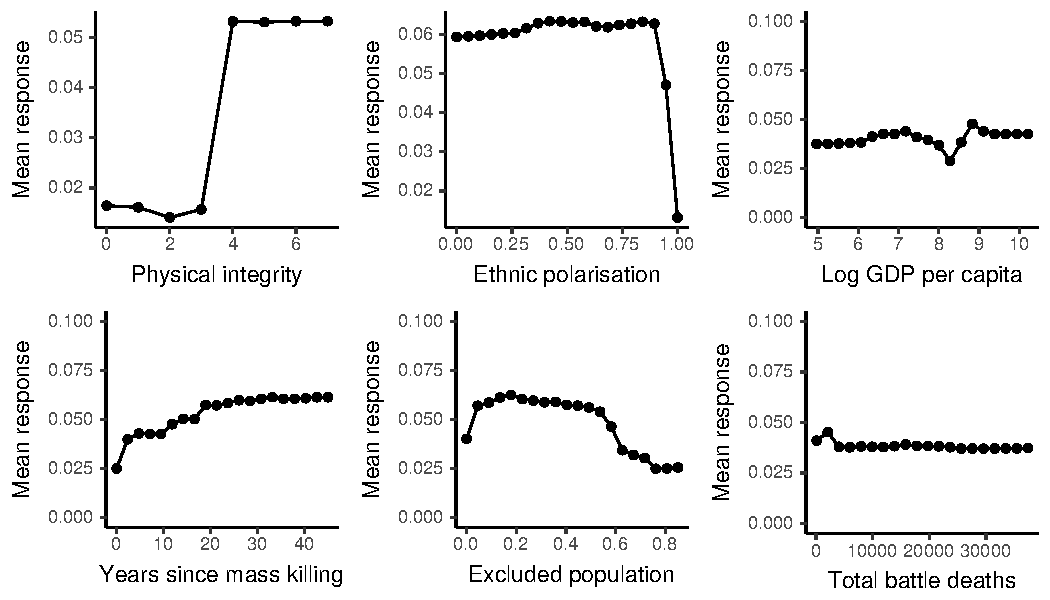
\includegraphics[width=\textwidth, height=9cm]{images/drfdpp3.pdf}
\caption{Partial Dependence Plots -- Mass Killings during Civil Wars (COW data)}
\label{fig:drfdpp3}
\end{center}
\end{figure}


\begin{figure}[h!]
\begin{center}
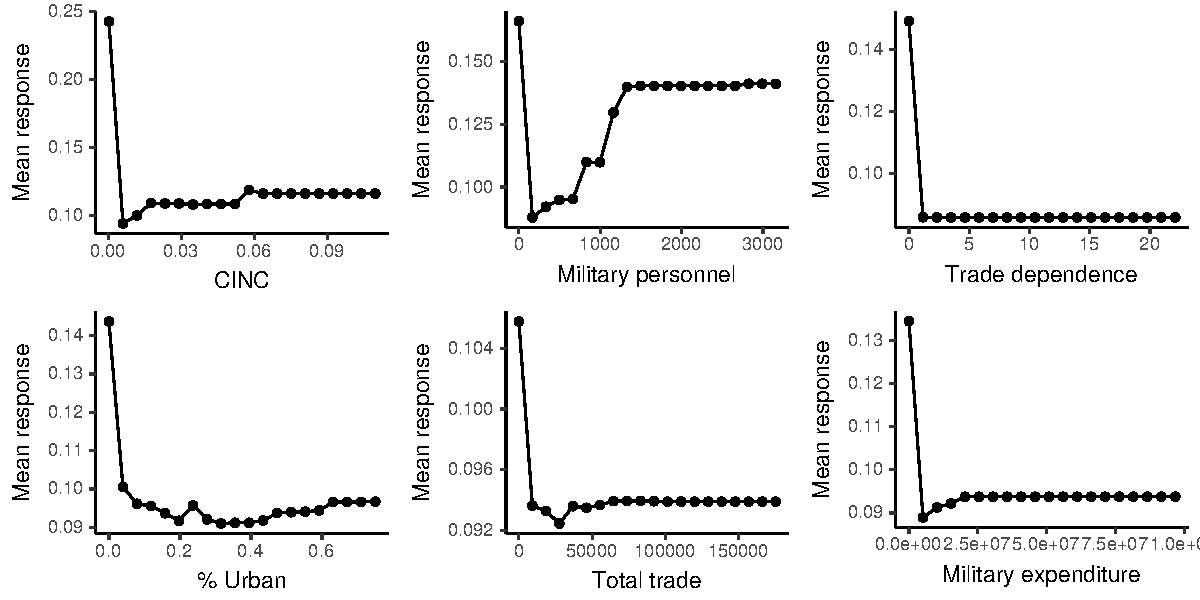
\includegraphics[width=\textwidth, height=9cm]{images/drfdpp4.pdf}
\caption{ Partial Dependence Plots -- Mass Killings during Civil Wars (Cederman et al. data)}
\label{fig:drfdpp4}
\end{center}
\end{figure}

\newpage

When using the COW data, we find that GDP per capita and total battle deaths have little influence in the likelihood of mass killings, and years since the last state-led atrocity increases the chances of a future event, a result we have also seen in the EBA models. As expected, higher levels of abuse against the physical integrity of citizens are associated with mass killings. Ethnic polarisation and the threshold of excluded population have a somewhat constant effect in our estimations, yet both show a sharp decline in probability when they reach their maximum levels. This provides more evidence to the idea that when certain groups are able to concentrate power, they tend not to resort to mass-scale violence as a political means.

Our last model concerns the onset of ethnic conflicts as defined by \citet{cederman2010ethnic}. The graphs show ethnic wars operate with a different dynamics than other armed conflicts. We see that an increase in all the most important predictors have a large negative impact on the likelihood of mass killings, thus we conclude that poor, unstable countries are more prone mass killings during ethnic conflicts.

\section{Additional Tests}
\label{sec:additional-tests4}

We estimate a set of additional regressions to assess the robustness of our main findings. In regard to the EBA, we include 10 variants of our original model. All of them largely confirm our prior results. First, we varied the number of covariates included in each regression to 3 and 5 while keeping the $M$ set of 3 variables included in every model, that is, the natural logarithm of GDP per capita, the Polity IV index, and a linear time trend since the last episode of state-sponsored violence. The results are identical to the main model when we add 3 control variables at a time. The same covariates discussed above remain significant and with the same sign: log of GDP per capita (negative), post-Cold War period (negative), previous riots (positive), civil war onset and ongoing indicators as measured by the UCDP data set (both positive), Polity IV squared (negative), and ethnic diversity (negative). When 5 control variables are added to every model, three variables have a CDF(0) of 0.9 or higher. They are the natural logarithm of GDP per capita, civil war onset (UCDP), previous riots, and the dummy indicating the post-Cold War period. Ethnic fractionalisation and Polity IV squared become marginally significant with a CDF(0) of about 0.88.

Second, we place different restrictions on the variance inflation factor (VIF) to test whether multicollinearity is driving our results. The test is similar to that employed by Bell (2015). While in the main analysis we use a VIF of 7, in the additional analyses we include a conservative VIF of 2.5, a less strict value of 10, and a model without any restriction. The results are unchanged. The two models with different values of VIF show identical results to the results displayed in table \ref{tab:eba1}. In the model with no VIF restriction, however, ethnic fractionalisation fails to meet our threshold by a very small margin. The CDF(0) of that covariate is 0.897, very close to the required value of 0.9.

We also estimate our models using logit and probit regressions. In order to deal with the issue of complete separation \citep{bell2015questioning,zorn2005solution} we follow \citet{gelman2008weakly} and add a weakly informative prior distribution to the coefficients. We first scaled the non-binary variables to have a mean of 0 and a standard deviation of 0.5, then we added a Cauchy distribution with center 0 and scale 2.5. The probit regressions use a scale of $2.5 \times 1.6$, which is also recommended by the authors \citep{arm2017rpackage}.

In both cases, the logarithm of GDP per capita, post-Cold War period, previous riots, and Polity IV squared remain significant. In contrast, ethnic fractionalisation and former conflict as measured by the UCDP data set are again close to the 0.9 significance level. 

In regard to random forests, grid searches are themselves a data-driven selection of many possible machine learning models, thus it is not strictly necessary to run a batch of additional tests. Nevertheless, we performed a series of grid searches using three different seeds obtained from \texttt{Random.Org} to estimate how the choice of different starting numbers would influence the model outcomes. The output of those models are largely comparable.

As a last set of robustness models, we estimate the same regressions using Harff's (\citeyear{harff2003no}) indicator of genocide and politicide. No variable appear as significant in our EBA models for genocide or politicide onset in peacetime. When we limit our sample to civil war years, the Post-Cold War period is again negatively correlated with the outcome when using the Correlates of War data set. Additionally, excluded population has a negative sign in more than 90\% of the models using both Correlates of War’s and Cederman et al's (\citeyear{cederman2010ethnic}) indicators of conflict. Displaced population also has a negative effect in the Correlates of War data set. During ethnic conflicts, our dummy variable for political assassinations has a negative impact on the onset of genocides. Overall, we conclude then that the significant covariate of genocide and politicide onset differ significantly from those of more general forms of government mass violence. Finally, the machine learning models are comparable to the ones we present above, with a similar set of variables appearing in the random forest estimations. The complete results are available in the appendix.

\section{Conclusion}
\label{sec:conclusion4}

In this paper, we apply extreme bounds analysis and distributed random forests to estimate the robustness and predictive ability of 40 variables that have been pointed out as potential determinants of mass killings. We find that from all variables we employ, GDP per capita is the covariate that appears statistically significant more often in our models. In the EBA estimations, we see that the level of democracy, and the post-Cold War period are negatively associated with our dependent variable, whereas ethnic diversity, civil wars, and previous political turmoils increase the likelihood of those events. When we run a machine learning algorithm to estimate out-of-sample predictive performance, GDP per capita and years since last mass killings again appear as important predictors, and variables related to military capabilities and the composition of the population are included in most models. In a nutshell, our tests provide strong evidence in favour of two well-established findings in the specialised literature: Mass killings are unlikely to happen in rich, stable countries and there is a positive association between several types of political conflict, such as previous riots, civil wars and government atrocities.

Nevertheless, there is considerable heterogeneity in some of our findings. Mass killings are rare outcomes, so it is possible that our analysis does not capture all variables that explain the onset of large-scale violence, or that the effect of predictors vary across time and space \citep[8]{bell2015examining}. Additionally, the findings point out that mass killings may have different causes according to the context in which they erupt, so a general theory of state atrocities may obscure important details in our understanding of the root causes of state killings. 

Yet we see this diversity of outcomes under a positive light. The findings presented in this text suggest new avenues for research, and we believe they also highlight the importance of scholars moving from purely correlational, cross-country regressions to other methods that can yield more robust predictions and causal explanations. For instance, why are mass killings in ethnic conflicts correlated with a different set of variables than in armed conflicts in general? Would the results remain robust had scholars decided to code ethnic conflicts in another way? More theoretical advancement would also be welcome. Given that GDP per capita is negatively correlated to state atrocities in virtually every model, it would be interesting to unpack the causal mechanisms by which it operates by testing more specific mechanisms. Disaggregated data can also be of great help to further current research on genocides, politicide, and mass killings.

In terms of practical implications, the results indicate that regime change and pro-growth economic policies are the most efficient ways to prevent mass killings. The international community can therefore play a role in deterring leaders from using force against their own population, either by offering support for domestic opposition groups, intervening, or by fostering economic development. Although costly in the short run, these measures would substantially decrease the likelihood of state violence by breaking the ``conflict trap'' in which past conflicts create the condition for new ones \citep{collier2003breaking}. 

\section{Appendix} 
\label{sec:mk-appendix}

\subsection{Variable Selection}
\label{sec:mk-vs}

This appendix contains all required information to replicate the numerical analyses presented in the paper. We present a series of histograms with the coefficient distribution of every variable included in our EBA models. Robust variables  (CDF(0) $> 0.9$) are described in further detail in the tables below. 

The complete results can also be retrieved from data included at the following GitHub repository: \href{https://github.com/danilofreire/mass-killings}{https://github.com/danilofreire/mass-killings}. \textt{R} code is available in section \ref{sec:mk-code}. The analyses were conducted on \texttt{R} version 3.4.4 (15-03-2018) and Ubuntu 16.04.4 LTS.

\subsection{Descriptive Statistics}
\label{sec:mk-ds}

\begin{table}[!htbp] \centering 
  \caption{Descriptive Statistics} 
  \label{tab:mk-ds} 
\footnotesize 
\begin{tabular}{@{\extracolsep{5pt}}lccccc} 
\\[-1.8ex]\hline 
\hline \\[-1.8ex] 
Statistic & \multicolumn{1}{c}{N} & \multicolumn{1}{c}{Mean} & \multicolumn{1}{c}{St. Dev.} & \multicolumn{1}{c}{Min} & \multicolumn{1}{c}{Max} \\ 
\hline \\[-1.8ex] 
Country code & 9,162 & 452.84 & 247.74 & 2 & 950 \\ 
Year & 9,162 & 1,983.56 & 18.77 & 1,945 & 2,013 \\ 
Mass killing onset & 9,162 & 0.01 & 0.11 & 0 & 1 \\ 
Years since last mass killing & 9,162 & 23.81 & 17.71 & 0 & 68 \\ 
Years since last mass killing squared & 9,162 & 880.44 & 1,086.13 & 0 & 4,624 \\ 
Years since last mass killing cubed & 9,162 & 39,339.21 & 65,025.39 & 0 & 314,432 \\ 
UCDP civil war onset & 8,733 & 0.02 & 0.14 & 0 & 1 \\ 
UCDP civil war ongoing & 8,733 & 0.15 & 0.36 & 0 & 1 \\ 
COW civil war onset & 8,160 & 0.01 & 0.12 & 0 & 1 \\ 
COW civil war ongoing & 8,160 & 0.07 & 0.25 & 0 & 1 \\ 
Ethnic war start & 7,760 & 0.01 & 0.12 & 0 & 1 \\ 
Ethnic war ongoing & 7,760 & 0.11 & 0.31 & 0 & 1 \\ 
Assassination dummy & 8,991 & 0.08 & 0.27 & 0 & 1 \\ 
Democracy dummy & 8,991 & 0.37 & 0.48 & 0 & 1 \\ 
Ethnic diversity (ELF) & 6,981 & 0.41 & 0.31 & 0 & 1 \\ 
Mountainous Terrain & 7,358 & 2.14 & 1.43 & 0.00 & 4.56 \\ 
Population & 8,293 & 32,993.61 & 112,886.40 & 118.21 & 1,324,353.00 \\ 
Real GDP & 8,293 & 215,317.70 & 804,827.20 & 129.68 & 13,193,478.00 \\ 
Ln of real GDP per capita & 8,293 & 8.25 & 1.20 & 4.89 & 13.36 \\ 
Real GDP per capita & 8,293 & 8,104.20 & 18,376.73 & 132.82 & 632,239.50 \\ 
Polity IV & 8,558 & 0.42 & 7.50 & $-$10 & 10 \\ 
Polity IV squared & 8,558 & 56.35 & 32.59 & 0 & 100 \\ 
Excluded population & 6,981 & 0.16 & 0.22 & 0.00 & 0.98 \\ 
Discriminated population & 6,981 & 0.06 & 0.15 & 0.00 & 0.98 \\ 
Polarisation (all groups/main group) & 6,981 & 0.70 & 0.26 & 0.05 & 1 \\ 
Polarisation (all groups/population) & 6,981 & 0.63 & 0.32 & 0 & 1 \\ 
Polarisation (included groups/population) & 5,610 & 0.64 & 0.32 & 0 & 1 \\ 
Polarisation (included groups/main group) & 6,981 & 0.23 & 0.35 & 0 & 1 \\ 
Discriminated dummy & 6,981 & 0.35 & 0.48 & 0 & 1 \\ 
Interstate war & 8,159 & 0.04 & 0.19 & 0 & 1 \\ 
Military expenditure & 8,290 & 4,607,120 & 27,785,906 & 0 & 693,600,000 \\ 
Military personnel & 8,620 & 176.70 & 520.90 & 0 & 12,500 \\ 
Percent urban population & 8,767 & 0.22 & 0.17 & 0.00 & 1.51 \\ 
Post-Cold War & 8,991 & 0.40 & 0.49 & 0 & 1 \\ 
Coup dummy & 8,587 & 0.05 & 0.21 & 0 & 1 \\ 
Riot dummy & 8,991 & 0.16 & 0.36 & 0 & 1 \\ 
War with territory aims & 8,924 & 0.07 & 0.26 & 0 & 1 \\ 
Total trade & 8,174 & 53,804.01 & 222,209.90 & 0.80 & 4,825,363.00 \\ 
Trade dependence & 7,670 & 0.26 & 0.69 & 0.0001 & 22.11 \\ 
Militias & 4,097 & 0.22 & 0.42 & 0 & 1 \\ 
Physical integrity & 4,499 & 4.73 & 2.31 & 0 & 8 \\ 
CINC & 8,767 & 0.01 & 0.02 & 0.00 & 0.38 \\ 
Total battle deaths & 714 & 6,050.86 & 24,404.78 & 100 & 350,000 \\  
Guerrilla dummy & 714 & 0.81 & 0.40 & 0 & 1 \\ 
Regime transition & 1,221 & $-$4.24 & 41.50 & $-$77 & 99 \\ 
\hline \\[-1.8ex] 
\end{tabular} 
\raggedright{\newline \textit{Note}: All independent variables were lagged one year.}
\end{table} 
\normalsize

\newpage

\subsection{Extreme Bounds Analysis Extensions}
\label{sec:mk-ebae}

\subsubsection{Complete Results}

Here we present a series of histograms with the distribution of coefficients of all variables of the main EBA model. There are 36 variables in total, of which seven are robust: Log GDP per capita, post-Cold War period, onset and ongoing civil wars (measured by the UCDP), previous riots, ethnic diversity and the squared term of the Polity IV index.

\vspace{1cm}

\begin{table}[H]
\centering
\begin{tabular}{lrrrrr}
\hline
\textbf{Variable} & \textbf{Avg. $\beta$} & \textbf{Avg. SE} & \textbf{$\%$ Sig.} & \textbf{CDF(0)} & \textbf{Models} \\ \hline
\textit{Base variables} &  &  &  &  &  \\
Log GDP per capita & -0.0091 & 0.0052 & 76.055 & 0.9335 & 226707 \\
 &  &  &  &  &  \\
\textit{Additional variables} &  &  &  &  &  \\
Post-Cold War years & -0.0133 & 0.0085 & 72.845 & 0.9472 & 35614 \\
UCDP civil war onset & 0.0529 & 0.0321 & 52.378 & 0.9441 & 20854 \\
Previous riots & 0.0140 & 0.0100 & 56.242 & 0.9216 & 35614 \\
UCDP ongoing civil war & 0.0172 & 0.0115 & 65.652 & 0.9092 & 20854 \\
Ethnic diversity (ELF) & 0.0184 & 0.0137 & 56.674 & 0.9050 & 35614 \\
Polity IV squared & -0.0002 & 0.0001 & 61.206 & 0.9031 & 35614 \\ \hline
\end{tabular}
\caption{Extreme Bounds Analysis -- Mass killings (robust variables only)}
\label{tab:eba1}
\end{table}

\clearpage
\begin{sidewaysfigure}
    \centering
    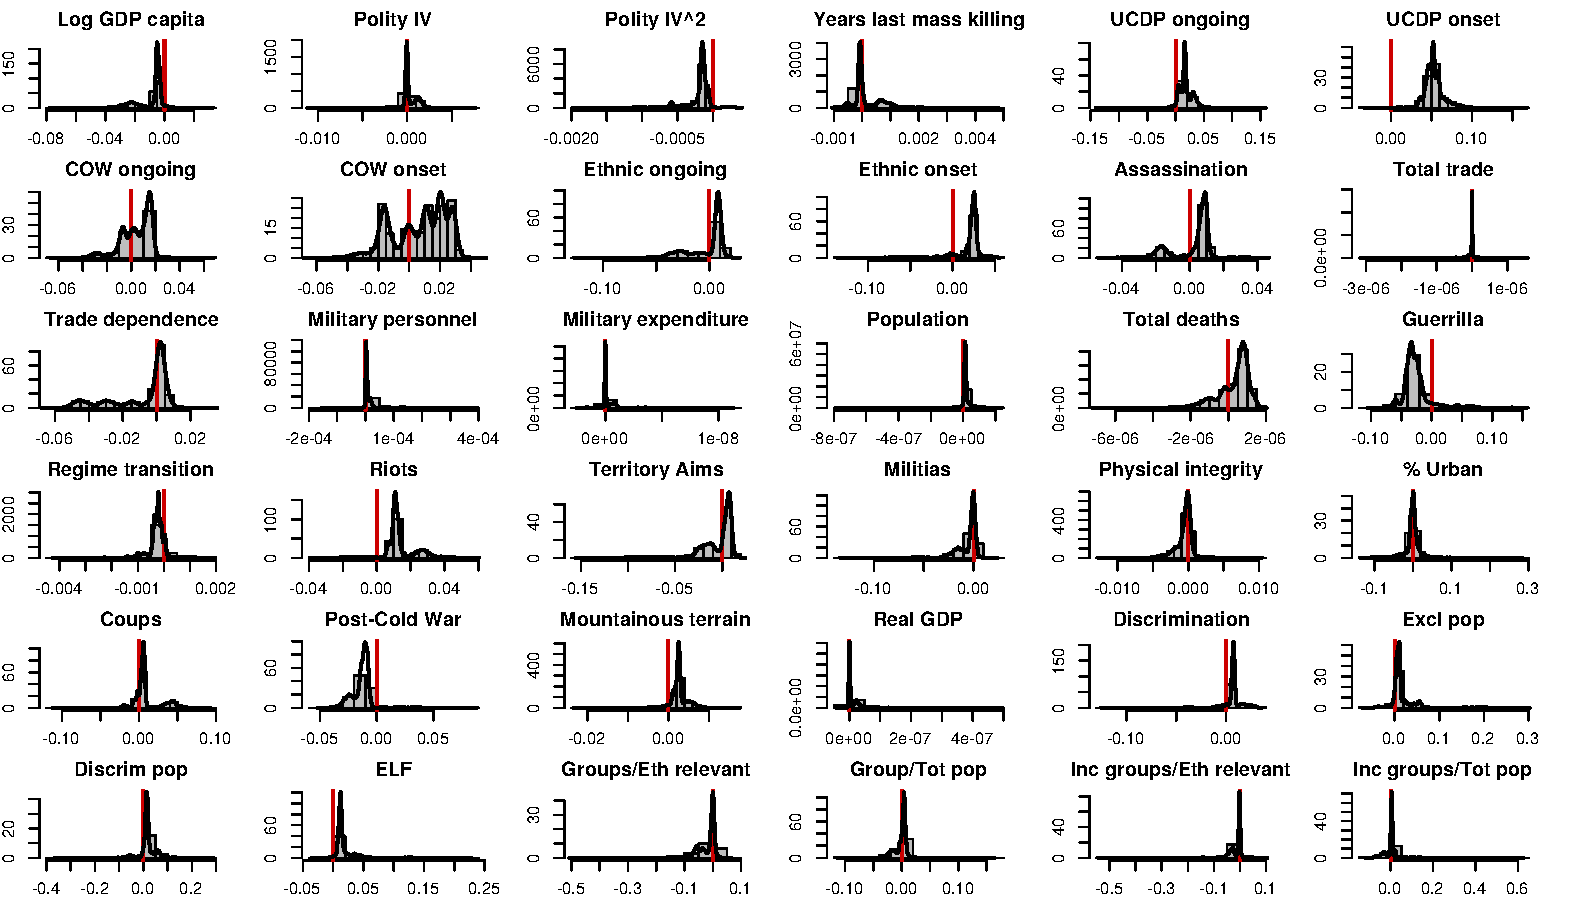
\includegraphics[width=\textwidth]{images/mk.pdf}
    \caption{Extreme Bounds Analysis -- Mass killings}
    \label{fig:hist-mk}
\end{sidewaysfigure}
\clearpage

\newpage

%%%%% Add models during civil wars

\subsubsection{Alternative Number of Variables}

The following table shows the results of an EBA model using 3 variable combinations at a time. The results are very similar to those reported in the paper, in which we used 4 variables in each model.

To speed up computational time, the models included in this appendix are based on 50,000 random draws from the full set of all possible regression models. \citet[819]{salaimartin2004determinants} argue that random sampling produces unbiased estimates of the regression coefficients, and as such can accelerate convergence of the results. The models presented in the paper, however, include the full set of regressions.

\begin{table}[H]
\centering
\begin{tabular}{lrrrrr}
\hline
\textbf{Variable} & \textbf{Avg. $\beta$} & \textbf{Avg. SE} & \textbf{$\%$ Sig.} & \textbf{CDF(0)} & \textbf{Models} \\ \hline
\textit{Base variables} &  &  &  &  &  \\
Log GDP per capita & 0.0082 & 0.0043 & 81.439 & 0.9504 & 40677 \\
 &  &  &  &  &  \\
\textit{Additional variables} &  &  &  &  &  \\
Post-Cold War years & -0.0121 & 0.0069 & 77.804 & 0.9609 & 5064 \\
UCDP civil war onset & 0.0523 & 0.0292 & 62.561 & 0.9574 & 3304 \\
Previous riots &0.0134 & 0.0084 & 65.936 & 0.9401 & 5064 \\
UCDP ongoing civil war & 0.0177 & 0.0094 & 72.367 & 0.9372 & 3304 \\
Polity IV squared & -0.0002 & 0.0001 & 66.035 & 0.9268 & 5064 \\ 
Ethnic diversity (ELF) & 0.0162 & 0.0110 & 70.794 & 0.9266 & 5064 \\\hline
\end{tabular}
\caption{EBA -- 3 variables in each regression model}
\label{tab:mk-3vars}
\end{table}

\clearpage
\begin{sidewaysfigure}
    \centering
    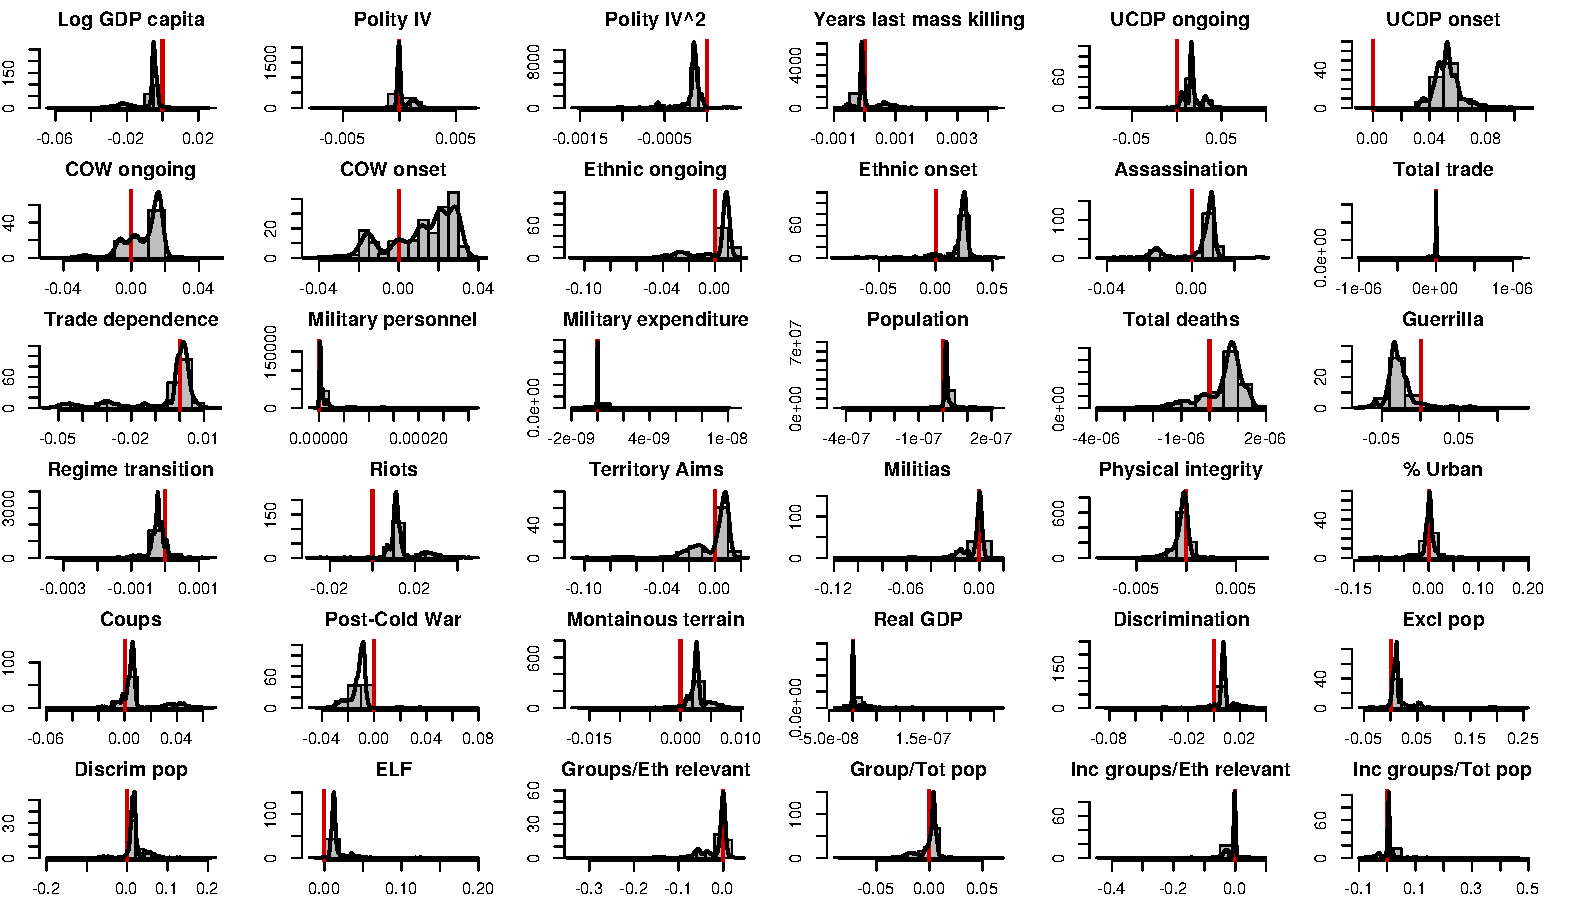
\includegraphics[width=\textwidth]{images/mk-3vars.pdf}
    \caption{EBA -- 3 variables in each regression model}
    \label{fig:hist-mk-3vars}
\end{sidewaysfigure}
\clearpage

Table \ref{tab:mk-5vars} presents the results for models with up 5 variables in each regressions. In contrast with the main EBA model, the indicators of UCDP ongoing civil wars, ethnic diversity, and Polity IV square drop out of significance. Their CDF(0) is 0.88, just marginally below our threshold of 0.9.

\vspace{1cm}

\begin{table}[!htpb]
\centering
\begin{tabular}{lrrrrr}
\hline
\textbf{Variable} & \textbf{Avg. $\beta$} & \textbf{Avg. SE} & \textbf{$\%$ Sig.} & \textbf{CDF(0)} & \textbf{Models} \\ \hline
\textit{Base variables} &  &  &  &  &  \\
Log GDP per capita & -0.010 & 0.006 & 70.806 & 0.9161 & 50000 \\
 &  &  &  &  &  \\
\textit{Additional variables} &  &  &  &  &  \\
Post-Cold War years & -0.014 & 0.010 & 68.496 & 0.9336 & 9532 \\
UCDP civil war onset & 0.053 & 0.035 & 44.784 & 0.9308 & 5100 \\
Previous riots & 0.015 & 0.012 & 47.988 & 0.9047 & 9569 \\\hline
\end{tabular}
\caption{EBA -- 5 variables in each regression model}
\label{tab:mk-5vars}
\end{table}

\clearpage
\begin{sidewaysfigure}
    \centering
    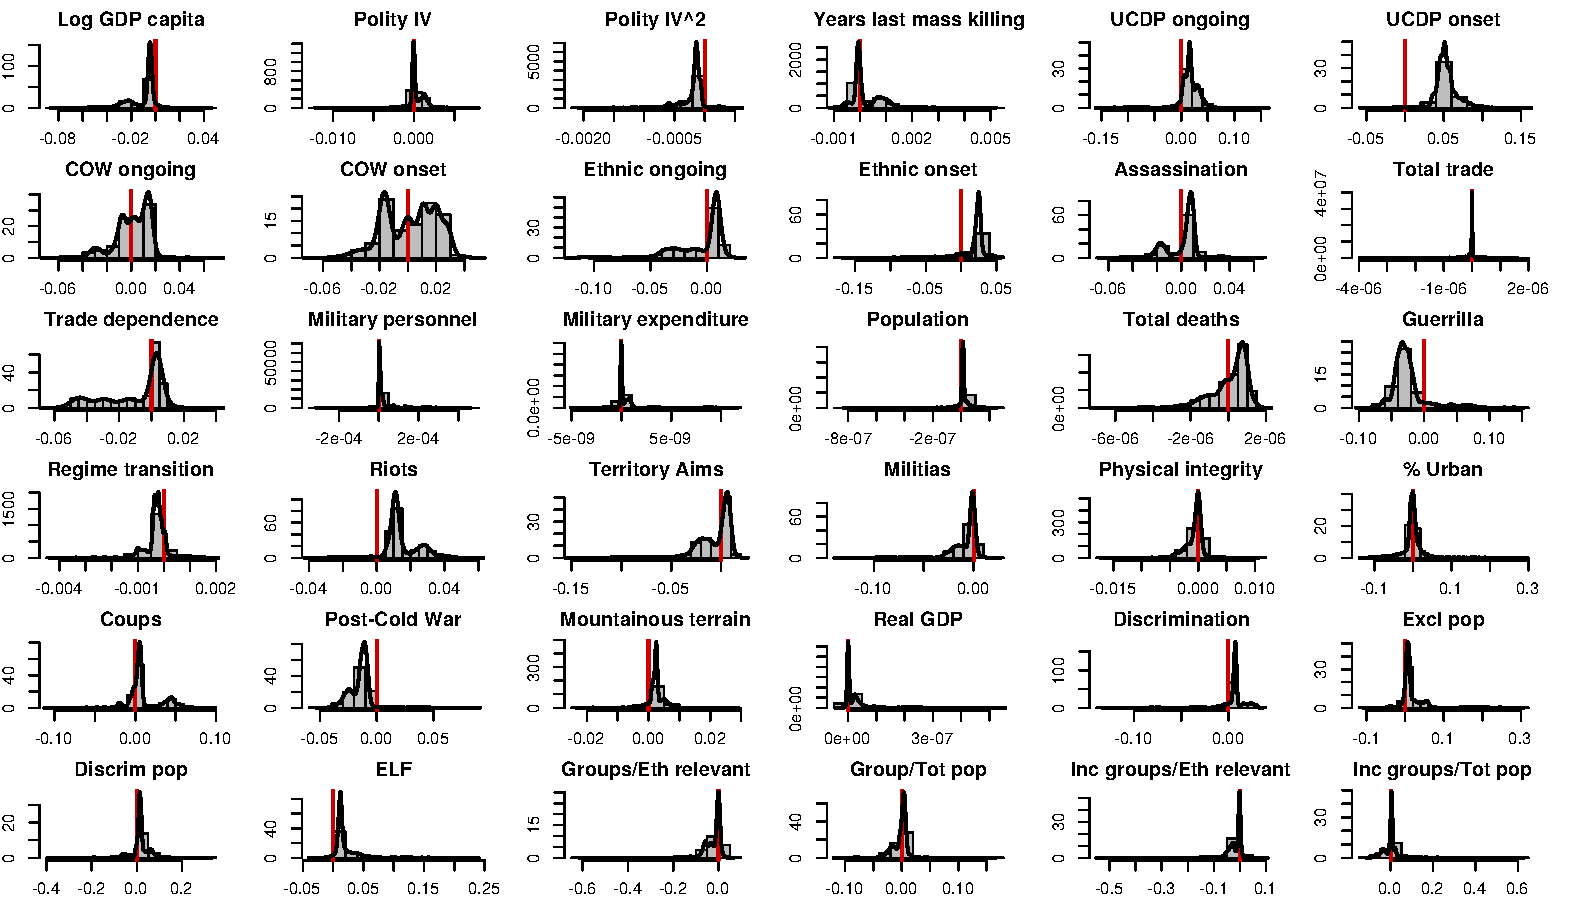
\includegraphics[width=\textwidth]{images/mk-5vars.pdf}
    \caption{EBA -- 5 variables in each regression model}
    \label{fig:hist-mk-5vars}
\end{sidewaysfigure}
\clearpage

\subsubsection{Alternative Variance Inflation Factors}

In this section, we estimate the EBA model with different values of Variance Inflation Factor (VIF), a measure of multicollinearity for linear models. There is no standard definition about what constitutes an acceptable VIF value, although researchers often use a value of 10 as rule of thumb to indicate strong multicollinearity \citep[674]{o2007caution}. Our original model used 7 as a cutoff, and here we employ 10 (less strict), a lower value of 2.5 (more conservative), and a model without any VIF value (no restriction). The results are essentially identical to those in the main model. In the model with no VIF restriction, however, ethnic fractionalisation fails to meet our threshold by a very small margin. The CDF(0) of that covariate is 0.897, very close to the required value of 0.9. 

\vspace{1cm}

\begin{table}[H]
\centering
\begin{tabular}{lrrrrr}
\hline
\textbf{Variable} & \textbf{Avg. $\beta$} & \textbf{Avg. SE} & \textbf{$\%$ Sig.} & \textbf{CDF(0)} & \textbf{Models} \\ \hline
\textit{Base variables} &  &  &  &  &  \\
Log GDP per capita & -0.0091 & 0.0052 & 76.354 & 0.9343 & 50000 \\
 &  &  &  &  &  \\
\textit{Additional variables} &  &  &  &  &  \\
Post-Cold War years & -0.0134 & 0.0084 & 73.540 & 0.9495 & 7929 \\
UCDP civil war onset & 0.0529 & 0.0322 & 52.141 & 0.9438 & 4553 \\
Previous riots & 0.0140 & 0.0100 & 56.433 & 0.9216 & 7772 \\
UCDP ongoing civil war & 0.0172 & 0.0113 & 66.013 & 0.9113 & 4587 \\
Ethnic diversity (ELF) & 0.0182 & 0.0136 & 56.872 & 0.9056 & 8076 \\
Polity IV squared & -0.0002 & 0.0001 & 60.791 & 0.9021 & 7835 \\ \hline
\end{tabular}
\caption{EBA -- VIF 10 (less strict)}
\label{tab:eba1}
\end{table}


\clearpage
\begin{sidewaysfigure}
    \centering
    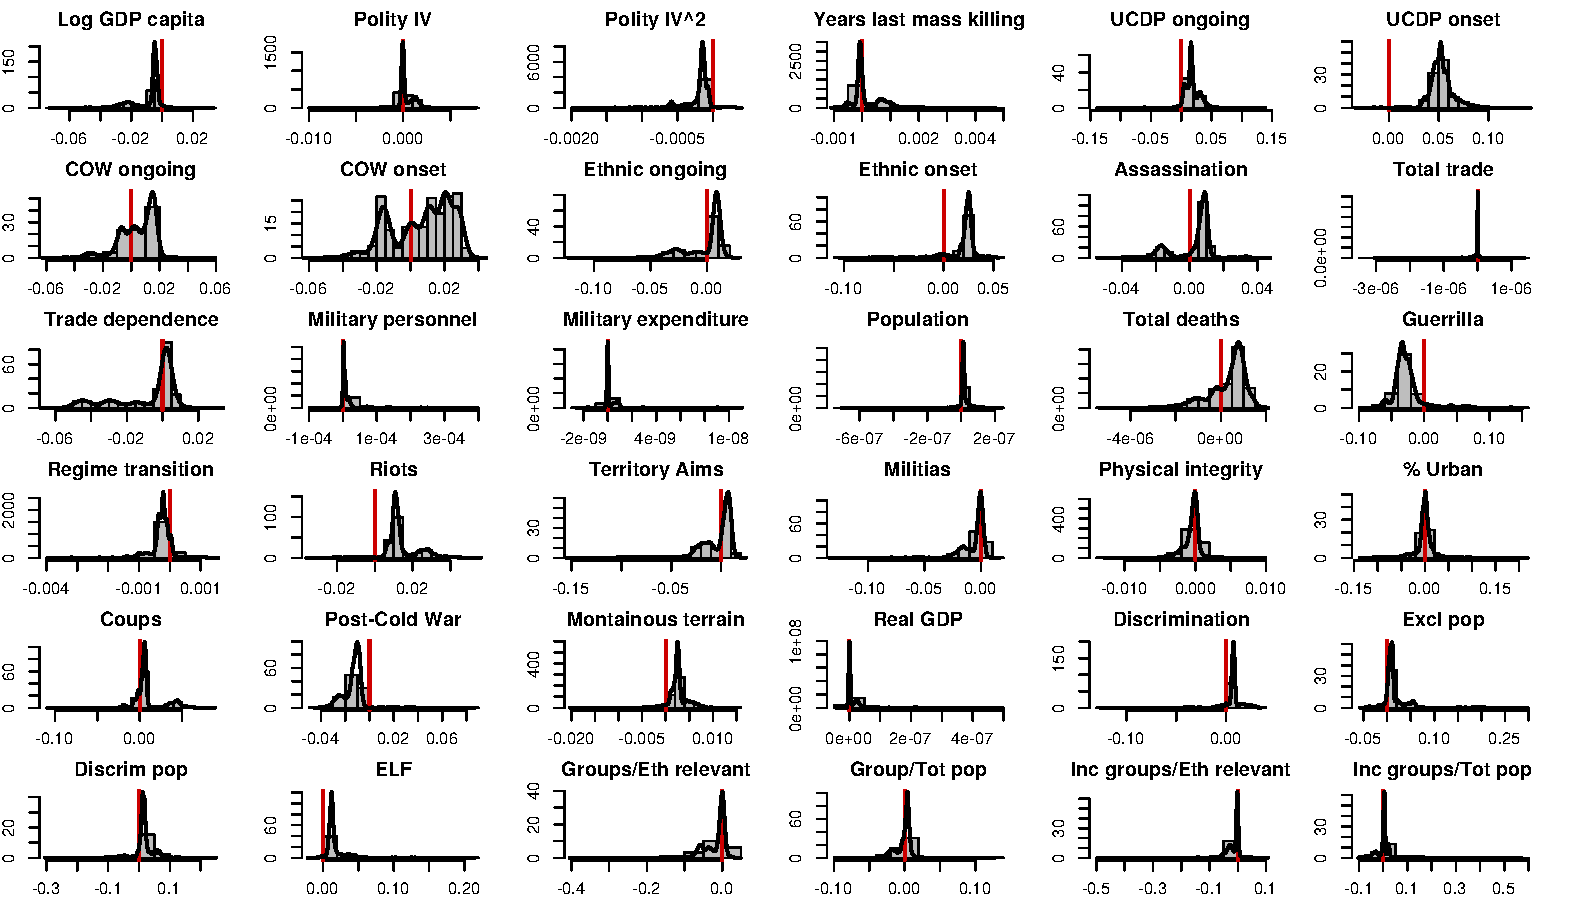
\includegraphics[width=\textwidth]{images/mk-high-vif.pdf}
    \caption{EBA -- VIF 10 (less strict)}
    \label{fig:hist-mk-high-vif}
\end{sidewaysfigure}
\clearpage

\vspace{1cm}

\begin{table}[H]
\centering
\begin{tabular}{lrrrrr}
\hline
\textbf{Variable} & \textbf{Avg. $\beta$} & \textbf{Avg. SE} & \textbf{$\%$ Sig.} & \textbf{CDF(0)} & \textbf{Models} \\ \hline
\textit{Base variables} &  &  &  &  &  \\
Log GDP per capita & -0.0090 & 0.0051 & 76.055 & 0.9343 & 49620 \\
 &  &  &  &  &  \\
\textit{Additional variables} &  &  &  &  &  \\
Post-Cold War years & -0.0132 & 0.0084 & 72.845 & 0.9490 & 7929 \\
UCDP civil war onset & 0.0529 & 0.0322 & 52.378 & 0.9438 & 4553 \\
Previous riots & 0.0141 & 0.0101 & 56.242 & 0.9199 & 7772 \\
UCDP ongoing civil war & 0.0174 & 0.0114 & 65.652 & 0.9103 & 4587 \\
Ethnic diversity (ELF) & 0.0184 & 0.0137 & 56.674 & 0.9054 & 8076 \\
Polity IV squared & -0.0002 & 0.0001 & 61.206 & 0.90267 & 7835 \\ \hline
\end{tabular}
\caption{EBA -- VIF 2.5 (more conservative)}
\label{tab:eba1}
\end{table}

\clearpage
\begin{sidewaysfigure}
    \centering
    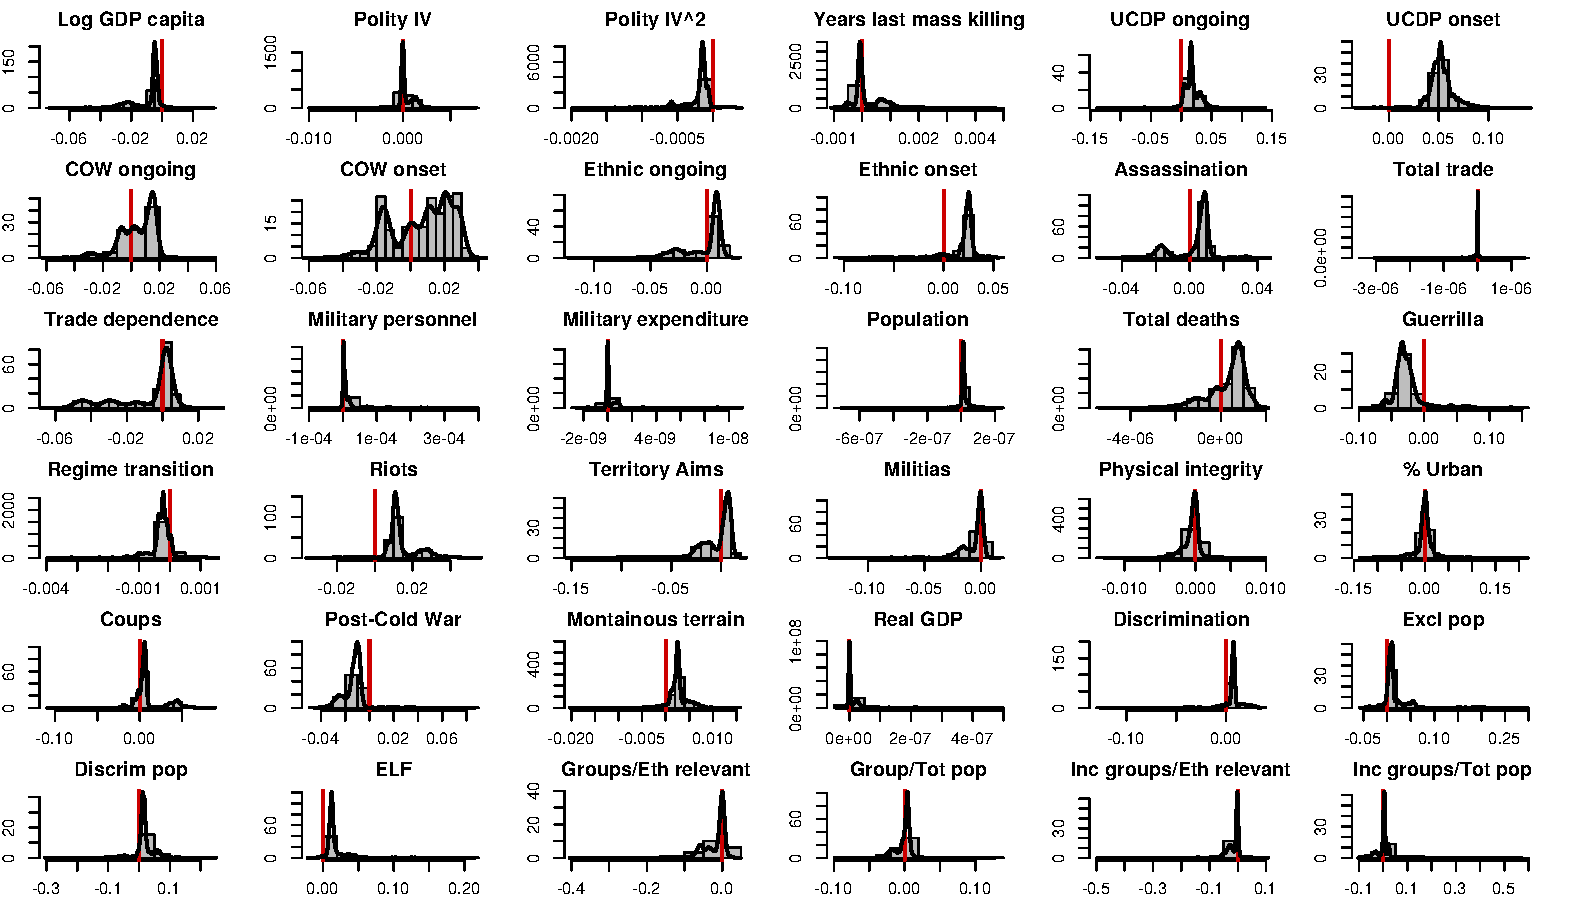
\includegraphics[width=\textwidth]{images/mk-high-vif.pdf}
    \caption{EBA -- VIF 2.5 (more conservative)}
    \label{fig:hist-mk-high-vif}
\end{sidewaysfigure}
\clearpage






















\newpage

\subsubsection{Generalised Linear Models}

We estimate the same EBA with logit and probit in addition to the linear probability model reported above. The results are 

\subsection{Random Forest Extensions}
\label{sec:mk-rfe}


\subsection{\texttt{R} Code}
\label{sec:mk-code}

The code below reproduces the analyses included here.

\singlespacing
\small
\begin{verbatim}
######################
### Data Wrangling ###
######################

\end{verbatim}


\doublespacing
\normalsize